% !TeX program = lualatex
% !TeX encoding = UTF-8
% !TeX spellcheck = fr_FR
%
% ==============================================================================
% TP4 — Défense Active avec Snort (IDS/IPS)
% Rapport complet (style identique TP1–TP3)
% ==============================================================================
\documentclass[12pt,a4paper,openany]{report}

% ==============================================================================
% 1. MOTEUR & LANGUE (Spécifique LuaLaTeX)
% ==============================================================================
\usepackage{fontspec}
\usepackage{polyglossia}
\setmainlanguage{french}
\setotherlanguage{english}

% ==============================================================================
% 2. MISE EN PAGE & STRUCTURE
% ==============================================================================
\usepackage{geometry}
\geometry{left=2.5cm, right=2.5cm, top=3cm, bottom=3cm, headheight=30pt}

\usepackage{fancyhdr}
\usepackage{titlesec}
\usepackage{tocloft}
\usepackage{titletoc}

% ==============================================================================
% 3. TYPOGRAPHIE & TEXTE
% ==============================================================================
\usepackage{setspace}
\usepackage{xcolor}
\usepackage{csquotes}
\usepackage{enumitem}
\usepackage{indentfirst}
\usepackage{hyphenat}
\usepackage[skins]{tcolorbox}

% ==============================================================================
% 4. MATHÉMATIQUES & SYMBOLES
% ==============================================================================
\usepackage{amsmath}
\usepackage{amssymb}
\usepackage{amsfonts}
\usepackage{mathtools}
\usepackage{bm}

% ==============================================================================
% 5. GRAPHISMES & DIAGRAMMES
% ==============================================================================
\usepackage{graphicx}
\usepackage{tikz}
\usetikzlibrary{positioning, shapes.geometric, arrows.meta, calc}
\usepackage{pgfplots}
\pgfplotsset{compat=1.18}
\usepackage{caption}
\usepackage{subcaption}
\usepackage{float}

% ==============================================================================
% 6. TABLEAUX
% ==============================================================================
\usepackage{booktabs}
\usepackage{longtable}
\usepackage{array}
\usepackage{multirow}
\usepackage{tabularx}
\usepackage{colortbl}

% ==============================================================================
% 7. CODE SOURCE & LISTINGS
% ==============================================================================
\usepackage{listings}
\usepackage{lstautogobble}

% ==============================================================================
% 8. LIENS & RÉFÉRENCES
% ==============================================================================
\usepackage{hyperref}
\usepackage{bookmark}
\usepackage{url}
\usepackage{hypcap}

% ==============================================================================
% 9. UTILITAIRES DIVERS
% ==============================================================================
\usepackage{pdfpages}
\usepackage{imakeidx}
\usepackage{lastpage}
\usepackage{lipsum}

% ==============================================================================
% POLICES ET TYPOGRAPHIE
% ==============================================================================
\setmainfont{Latin Modern Roman}
\setsansfont{Latin Modern Sans}
\setmonofont{Latin Modern Mono}

% ==============================================================================
% COULEURS ET STYLE (Palette Professionnelle)
% ==============================================================================
\definecolor{primary}{RGB}{0,51,102}       % Bleu Nuit Profond
\definecolor{secondary}{RGB}{0,102,204}    % Bleu Plus Clair
\definecolor{accent}{RGB}{204,0,0}         % Rouge Accent
\definecolor{codebg}{RGB}{248,248,248}     % Gris Très Clair pour code
\definecolor{codekeyword}{RGB}{0,0,200}
\definecolor{codestring}{RGB}{163,21,21}
\definecolor{codecomment}{RGB}{0,128,0}
\definecolor{footergray}{RGB}{128,128,128}
\definecolor{logbgcolor}{RGB}{250,250,250}
% Table colors
\definecolor{tableheadbg}{RGB}{0,51,102}
\definecolor{tableheadfg}{RGB}{255,255,255}
\definecolor{tablerowalt}{RGB}{235,242,252}
\definecolor{tableborder}{RGB}{0,80,160}

% ==============================================================================
% EN-TÊTES ET PIEDS DE PAGE (FIXED)
% ==============================================================================
\pagestyle{fancy}
\fancyhf{}

\renewcommand{\headrulewidth}{0.4pt}
\renewcommand{\headrule}{\hbox to\headwidth{%
		\color{primary}\leaders\hrule height \headrulewidth\hfill}}
\renewcommand{\footrulewidth}{0.4pt}
\renewcommand{\footrule}{\hbox to\headwidth{%
		\color{primary}\leaders\hrule height \footrulewidth\hfill}}

\fancyhead[L]{\textcolor{primary}{\small\bfseries
		Architecture \& Sécurité des Réseaux \textbullet\ TP\,4}}
\fancyhead[R]{\textcolor{primary}{\small\bfseries
		ESTK \textbullet\ IDRS}}

% New conditional footer - checks if we're using gobble
\newif\ifshowpagenumbers
\showpagenumberstrue

\fancyfoot[C]{\textcolor{footergray}{\small%
		\ifshowpagenumbers%
		Page \thepage\ sur \pageref{LastPage}%
		\fi%
}}

\fancypagestyle{plain}{
	\fancyhf{}
	\renewcommand{\headrulewidth}{0pt}
	\renewcommand{\footrulewidth}{0.4pt}
	\renewcommand{\footrule}{\hbox to\headwidth{%
			\color{primary}\leaders\hrule height \footrulewidth\hfill}}
	\fancyfoot[C]{\textcolor{footergray}{\small%
			\ifshowpagenumbers%
			Page \thepage\ sur \pageref{LastPage}%
			\fi%
	}}
}

% Command to hide page numbers
\newcommand{\hidepagenumbers}{\showpagenumbersfalse\pagestyle{empty}}
\newcommand{\showpagenumbers}{\showpagenumberstrue\pagestyle{fancy}}

% ==============================================================================
% FORMATAGE DES TITRES
% ==============================================================================
\titleformat{\chapter}[display]
{\normalfont\huge\bfseries\color{primary}}{\chaptertitlename\ \thechapter}{20pt}{\Huge}
\titleformat{\section}
{\normalfont\Large\bfseries\color{primary}}{\thesection}{1em}{}
\titleformat{\subsection}
{\normalfont\large\bfseries\color{secondary}}{\thesubsection}{1em}{}

% ==============================================================================
% CONFIGURATION LISTINGS POUR LE CODE
% ==============================================================================
\lstset{
	basicstyle=\ttfamily\small,
	backgroundcolor=\color{codebg},
	keywordstyle=\color{codekeyword}\bfseries,
	stringstyle=\color{codestring},
	commentstyle=\color{codecomment}\itshape,
	frame=single,
	rulecolor=\color{primary},
	breaklines=true,
	breakatwhitespace=true,
	showstringspaces=false,
	captionpos=b,
	numbers=left,
	numberstyle=\tiny\color{gray},
	numbersep=5pt,
	tabsize=4,
	extendedchars=true,
	inputencoding=utf8,
	autogobble=true
}

\lstdefinestyle{logstyle}{
	basicstyle=\ttfamily\footnotesize,
	backgroundcolor=\color{logbgcolor},
	frame=none,
	breaklines=true,
	showstringspaces=false,
	captionpos=b,
	autogobble=true
}

% ==============================================================================
% COMMANDE TABLE STYLISÉE
% ==============================================================================
\newcommand{\tableheadcolor}{\rowcolor{tableheadbg}}

% ==============================================================================
% MÉTADONNÉES HYPERREF
% ==============================================================================
\hypersetup{
	colorlinks=true,
	linkcolor=primary,
	filecolor=magenta,
	urlcolor=secondary,
	pdftitle={Rapport Technique : Défense Active avec Snort (IDS/IPS) - TP4},
	pdfauthor={Yasser Bella, Oussama El Habti, Salma El Habti},
	pdfsubject={Cybersécurité Défensive : IDS/IPS, Snort, Alerting et Faux Positifs},
	pdfkeywords={Snort, IDS, IPS, pfSense, Emerging Threats, Signatures, Lateral Movement}
}

% ==============================================================================
% INTERLIGNE
% ==============================================================================
\onehalfspacing

% ==============================================================================
% DÉBUT DU DOCUMENT
% ==============================================================================
\begin{document}
	\sloppy
	
	% ------------------------------------------------------------------------------
	% PAGE DE TITRE (DESIGN PROFESSIONNEL)
	% ------------------------------------------------------------------------------
	\begin{titlepage}
		\thispagestyle{empty}
		
		% ── BARRE SUPÉRIEURE ────────────────────────────────────────────────
		\noindent
		\colorbox{primary}{%
			\parbox{\dimexpr\textwidth-2\fboxsep}{%
				\vspace{0.6cm}
				\centering
				{\large\bfseries\textcolor{white}{Cyberdéfense et Sécurité Offensive}}\\[0.6cm]
			}%
		}
		
		\vspace{1.5cm}
		\centering
		
		% ── LABEL TP ────────────────────────────────────────────────────────
		{\normalsize\bfseries\color{black!40}\MakeUppercase{Travaux Pratiques N\textsuperscript{o}4}}
		
		\vspace{0.8cm}
		
		% ── TITRE PRINCIPAL ─────────────────────────────────────────────────
		{\Huge\bfseries\color{primary}
			Défense Active avec\\[0.25cm]
			Snort (IDS/IPS)\par
		}
		
		\vspace{0.5cm}
		
		% ── LIGNE DÉCORATIVE ────────────────────────────────────────────────
		{\color{accent}\rule{7cm}{1.5pt}\par}
		
		\vspace{0.5cm}
		
		% ── SOUS-TITRE ──────────────────────────────────────────────────────
		{\large\color{black!60}
			Visibilité Réseau, Détection par Signatures\\[0.2cm]
			et Analyse d'Alertes sur une Infrastructure Segmentée\par
		}
		
		\vspace{2cm}
		
		% ── INFORMATIONS ÉTUDIANTS ──────────────────────────────────────────
		{\large
			\renewcommand{\arraystretch}{1.5}
			\begin{tabular}{c}
				\textbf{\color{primary}Équipe de Réalisation :}\\[0.3cm]
				Yasser \textsc{Bella} \\
				Oussama \textsc{El Habti} \\
				Salma \textsc{El Habti} \\[0.6cm]
				
				\textbf{\color{primary}Filière :} IDRS --- Infrastructure Digitale Réseau et Sécurité \\[0.3cm]
				\textbf{\color{primary}Année Universitaire :} 2025 -- 2026 \\
			\end{tabular}
		}
		
		\vfill
		
		% ── BARRE INFÉRIEURE (TECHNOLOGIES) ─────────────────────────────────
		\noindent
		\colorbox{primary}{%
			\parbox{\dimexpr\textwidth-2\fboxsep}{%
				\vspace{0.35cm}
				\centering
				{\small\textcolor{white}{%
						pfSense 2.8.0
						\quad\textbullet\quad Snort (NIDS)
						\quad\textbullet\quad ET Open + Snort GPLv2}}\\[0.2cm]
				{\small\textcolor{white}{%
						Parrot Security OS
						\quad\textbullet\quad Ubuntu 25.04 (DMZ)
						\quad\textbullet\quad Windows XP SP3 (LAN)}}\\[0.35cm]
			}%
		}%
	\end{titlepage}
	
	% ------------------------------------------------------------------------------
	% PAGES LIMINAIRES
	% ------------------------------------------------------------------------------
	\hidepagenumbers
	\tableofcontents
	\newpage
	\listoffigures
	\listoftables
	\newpage
	
	% Restore page numbering for main content
	\cleardoublepage
	\showpagenumbers
	\pagenumbering{arabic}
	\setcounter{page}{1}
	
	% ==============================================================================
	% CHAPITRE 1 : INTRODUCTION
	% ==============================================================================
	\chapter{Introduction et Objectifs}
	
	\section{Contexte et Motivation}
	
	Ce TP4 conclut la progression TP1--TP3 en basculant du \textbf{mode offensif} (reconnaissance, exploitation, pivoting) vers la \textbf{défense active}. L'objectif est de démontrer qu'un pare-feu périmétrique seul, bien qu'indispensable, ne fournit pas une visibilité suffisante sur les attaques lorsque celles-ci empruntent des flux \textit{autorisés}.  
	
	Dans les TP précédents, une compromission du serveur DMZ a permis d'initier des actions de mouvement latéral vers le LAN (scan SMB/RDP, tentatives d'exploitation). Le pare-feu pfSense voyait principalement des connexions autorisées entre zones. Snort, au contraire, inspecte le contenu (\textit{payload}) et déclenche des alertes sur des signatures connues.
	
	\section{Objectifs Pédagogiques}
	
	À l'issue de ce TP4, l'étudiant doit être capable de :
	
	\begin{enumerate}[leftmargin=*]
		\item Distinguer \textbf{pare-feu}, \textbf{IDS} et \textbf{IPS}, et expliquer leurs rôles complémentaires.
		\item Installer et configurer \textbf{Snort} sur pfSense.
		\item Comprendre la \textbf{détection par signatures} et ses limites (attaques zero-day).
		\item Analyser des \textbf{alertes Snort} (horodatage, IP source/destination, ports, SID, description).
		\item Expliquer le concept de \textbf{faux positifs} et l'importance du \textbf{tuning}.
		\item Montrer la valeur d'un IDS pour la détection du \textbf{mouvement latéral} (lateral movement) dans un réseau segmenté.
	\end{enumerate}
	
	\section{Cadre Éthique et Légal}
	
	\begin{tcolorbox}[colback=accent!5!white, colframe=accent, title=\textbf{AVERTISSEMENT LÉGAL}]
		\textbf{Tous les tests ont été réalisés dans un environnement de laboratoire isolé et contrôlé.}
		
		Les techniques décrites ci-dessous ne doivent être utilisées que dans un cadre légal (pentest autorisé, lab de formation). Toute exploitation sans autorisation explicite est illégale.
	\end{tcolorbox}
	
	% ==============================================================================
	% CHAPITRE 2 : FONDEMENTS THÉORIQUES
	% ==============================================================================
	\chapter{Fondements Théoriques : Pare-feu vs IDS/IPS}
	
	\section{Pare-feu : Filtrage L3/L4}
	
	Un pare-feu traditionnel applique des règles de filtrage principalement basées sur les en-têtes réseau (\textbf{couches 3 et 4 du modèle OSI}) :
	\begin{itemize}
		\item adresses IP (source/destination),
		\item ports (source/destination),
		\item protocoles (TCP/UDP/ICMP),
		\item état des connexions.
	\end{itemize}
	
	Ainsi, si un flux est autorisé (ex : trafic SMB DMZ $\rightarrow$ LAN via une règle permissive), le pare-feu ne caractérise pas nécessairement le contenu comme malveillant.
	
	\section{IDS et IPS : Inspection approfondie (DPI)}
	
	\subsection{IDS (Intrusion Detection System)}
	Un IDS inspecte le trafic (\textbf{Deep Packet Inspection}) et génère des alertes dès qu'une signature correspond à un motif d'attaque connu. Il s'agit d'une défense \textbf{passive} : détection, journalisation, alerte.
	
	\subsection{IPS (Intrusion Prevention System)}
	Un IPS effectue la même inspection, mais peut \textbf{bloquer activement} le trafic (drop, reset, blocage IP). Il s'agit d'une défense \textbf{active} mais plus risquée en cas de faux positifs.
	
	\subsection{Comparaison synthétique}
	\begin{table}[H]
		\centering
		\renewcommand{\arraystretch}{1.5}
		\setlength{\arrayrulewidth}{0.5pt}
		\begin{tabular}{p{3cm} p{5.3cm} p{5.3cm}}
			\arrayrulecolor{tableborder}
			\hline
			\tableheadcolor
			\textcolor{tableheadfg}{\textbf{Technologie}} &
			\textcolor{tableheadfg}{\textbf{Principe}} &
			\textcolor{tableheadfg}{\textbf{Limites}} \\
			\hline
			\rowcolor{tablerowalt}
			Pare-feu &
			Filtrage IP/ports/protocoles (L3/L4) &
			Peu de visibilité sur le contenu, ne détecte pas forcément une attaque dans un flux autorisé \\
			IDS &
			DPI + signatures, alerte sans blocage &
			Dépend des signatures, bruit (faux positifs), pas d'action directe \\
			\rowcolor{tablerowalt}
			IPS &
			DPI + signatures + blocage actif &
			Risque d'interruption de services légitimes si mauvais tuning \\
			\hline
		\end{tabular}
		\caption{Comparaison Pare-feu vs IDS vs IPS}
		\label{tab:fw-ids-ips}
	\end{table}
	
	\section{Signatures Snort : Reconnaître l'ennemi}
	
	Snort compare en temps réel les flux réseau à une base de règles (signatures). Chaque règle est identifiée par un \textbf{SID} et contient :
	\begin{itemize}
		\item critères de correspondance (protocoles, ports, contenu),
		\item message (description),
		\item priorité (sévérité),
		\item classification.
	\end{itemize}
	
	\textbf{Limite :} la détection par signatures est très efficace sur les attaques connues, mais moins sur les attaques inconnues (zero-day) ou chiffrées.
	
	\section{Faux Positifs}
	Un \textit{faux positif} correspond à une alerte générée sur une activité légitime. Les conséquences :
	\begin{itemize}
		\item fatigue d'alerte,
		\item perte de temps d'analyse,
		\item risque de manquer une vraie attaque (faux négatif par distraction),
		\item en mode IPS : risque de coupure de service.
	\end{itemize}
	
	Le \textbf{tuning} consiste à ajuster catégories, seuils, listes de suppression, et exceptions pour réduire le bruit.
	
	% ==============================================================================
	% CHAPITRE 3 : ENVIRONNEMENT DE LAB
	% ==============================================================================
	\chapter{Environnement, Topologie et Plan d'Adressage}
	
	\section{Inventaire des Machines}
	
	\begin{table}[H]
		\centering
		\renewcommand{\arraystretch}{1.4}
		\setlength{\arrayrulewidth}{0.5pt}
		\begin{tabular}{>{\bfseries}p{3.5cm} p{3.2cm} p{2.8cm} p{3.2cm}}
			\arrayrulecolor{tableborder}
			\hline
			\tableheadcolor
			\textcolor{tableheadfg}{\textbf{Machine}} &
			\textcolor{tableheadfg}{\textbf{Rôle}} &
			\textcolor{tableheadfg}{\textbf{Zone}} &
			\textcolor{tableheadfg}{\textbf{OS}} \\
			\hline
			\rowcolor{tablerowalt}
			pfSense-Firewall & Pare-feu + IDS/IPS & WAN/DMZ/LAN & pfSense 2.8.0 \\
			Ubuntu DMZ & Serveur exposé / Pivot & DMZ & Ubuntu 25.04 \\
			\rowcolor{tablerowalt}
			Parrot Security & Machine attaquante & WAN & Parrot Security OS \\
			Windows XP Client & Cible secondaire & LAN & Windows XP SP3 \\
			\hline
		\end{tabular}
		\caption{Inventaire des Machines Virtuelles (TP4)}
		\label{tab:vm-inventory-tp4}
	\end{table}
	
	\section{Plan d'Adressage IP (Lab)}
	
	\begin{table}[H]
		\centering
		\renewcommand{\arraystretch}{1.4}
		\setlength{\arrayrulewidth}{0.5pt}
		\begin{tabular}{p{4cm} p{4cm} p{6cm}}
			\arrayrulecolor{tableborder}
			\hline
			\tableheadcolor
			\textcolor{tableheadfg}{\textbf{Zone}} &
			\textcolor{tableheadfg}{\textbf{Équipement}} &
			\textcolor{tableheadfg}{\textbf{Adresse IP}} \\
			\hline
			\rowcolor{tablerowalt}
			WAN (192.168.100.0/24) & pfSense WAN & 192.168.100.6 \\
			WAN (192.168.100.0/24) & Parrot (Attaquant) & 192.168.100.150 \\
			\rowcolor{tablerowalt}
			DMZ (192.168.10.0/24) & pfSense DMZ (GUI) & 192.168.10.1 \\
			DMZ (192.168.10.0/24) & Ubuntu DMZ & 192.168.10.100 \\
			\rowcolor{tablerowalt}
			LAN (192.168.20.0/24) & pfSense LAN & 192.168.20.1 \\
			LAN (192.168.20.0/24) & Windows XP & 192.168.20.50 \\
			\hline
		\end{tabular}
		\caption{Plan d'Adressage IP utilisé dans le TP4}
		\label{tab:ip-plan-tp4}
	\end{table}
	
	% ==============================================================================
	% CHAPITRE 4 : INSTALLATION ET CONFIGURATION DE SNORT
	% ==============================================================================
	\chapter{Déploiement de Snort sur pfSense (IDS Mode)}
	
	\section{Choix du Mode IDS (Détection seule)}
	
	\begin{tcolorbox}[colback=secondary!5!white, colframe=secondary, title=\textbf{Choix de conception : IDS Mode}]
		Dans ce laboratoire, Snort a été configuré en \textbf{mode IDS} (Blocking Mode \textbf{désactivé}).  
		
		\textbf{Justification :}
		\begin{itemize}
			\item Permettre la reproduction des attaques du TP3 (exploitation, pivoting) sans interruption.
			\item Collecter des alertes exploitables pour analyse.
			\item Éviter des coupures de service dues à des faux positifs.
		\end{itemize}
	\end{tcolorbox}
	
	\section{Installation du paquet Snort}
	
	\textbf{Procédure :}
	\begin{enumerate}[leftmargin=*]
		\item Accès à l'interface pfSense : \url{https://192.168.10.1}
		\item Menu : \textbf{System > Package Manager > Available Packages}
		\item Recherche : \texttt{snort}
		\item Installation du paquet \textbf{Snort} puis confirmation.
	\end{enumerate}
	
	\section{Activation des sources de règles (Signatures)}
	
	Les sources suivantes ont été activées dans \textbf{Services > Snort > Global Settings} :
	\begin{itemize}
		\item \textbf{Snort GPLv2 Community Rules} (Talos certified subset).
		\item \textbf{Emerging Threats Open (ET Open)}.
	\end{itemize}
	
	\begin{figure}[H]
		\centering
		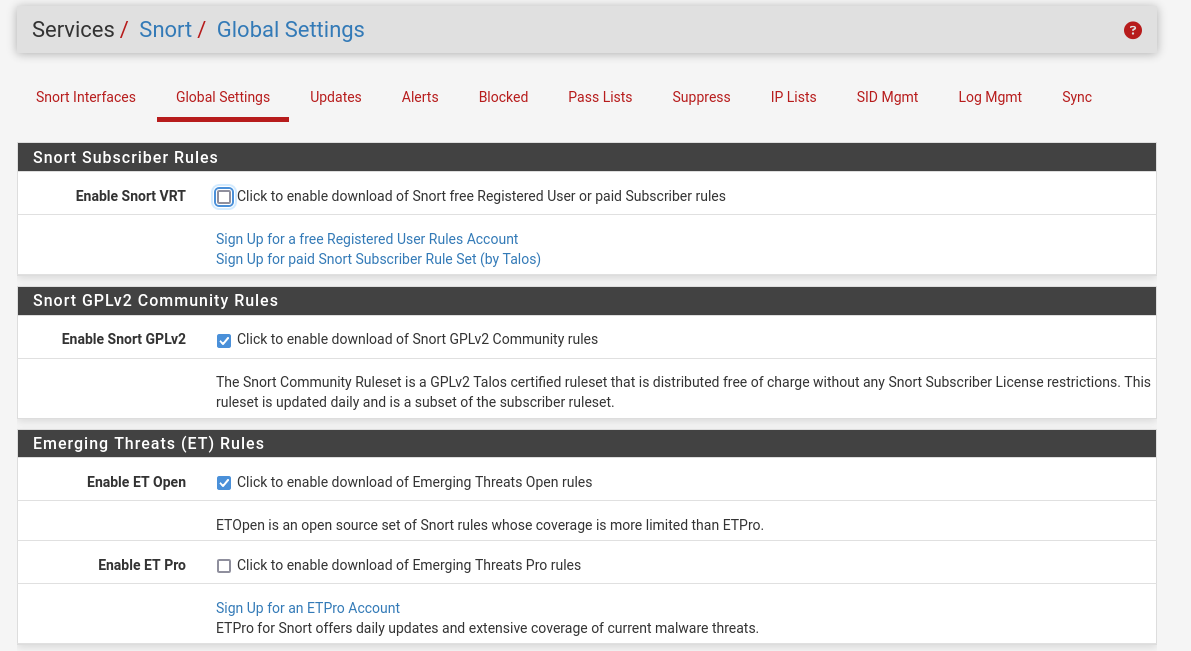
\includegraphics[width=0.98\textwidth]{screenshots/snort-global-settings.png}
		\caption{Snort : activation des sources de règles (GPLv2 + ET Open)}
		\label{fig:snort-global-settings}
	\end{figure}
	
	\section{Activation sur Interfaces (WAN + DMZ + LAN)}
	
	Snort a été activé sur trois interfaces afin de couvrir :
	\begin{itemize}
		\item \textbf{WAN :} détection d'attaques externes (reconnaissance, exploitation sur ports exposés).
		\item \textbf{DMZ :} surveillance de l'hôte pivot (serveur compromis).
		\item \textbf{LAN :} détection du mouvement latéral vers Windows XP (SMB/RDP).
	\end{itemize}
	
	\begin{figure}[H]
		\centering
		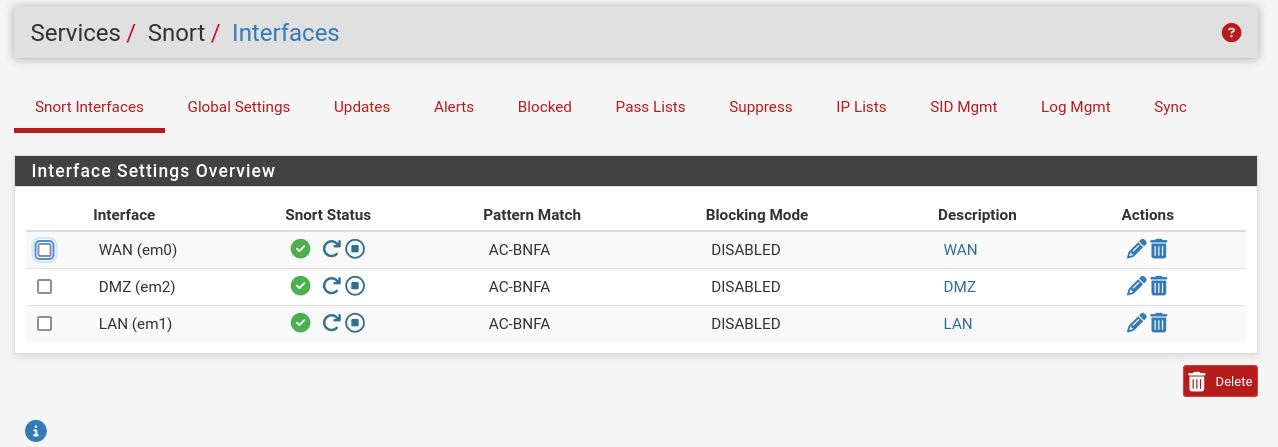
\includegraphics[width=0.98\textwidth]{screenshots/snort-interfaces.png}
		\caption{Snort Interfaces : WAN, DMZ et LAN en exécution (IDS mode, blocking disabled)}
		\label{fig:snort-interfaces}
	\end{figure}
	
	% ==============================================================================
	% CHAPITRE 5 : VALIDATION ET ANALYSE DES ALERTES
	% ==============================================================================
	\chapter{Validation : Détection WAN vs Mouvement Latéral LAN}
	
	\section{Principe de la démonstration ``Avant / Après''}
	
	L'objectif est de reproduire des événements similaires à ceux du TP3 et de vérifier que :
	\begin{itemize}
		\item un pare-feu seul ne fournit pas de contexte sur le contenu d'une attaque,
		\item Snort déclenche des alertes grâce à ses signatures,
		\item les alertes permettent de corréler \textbf{source}, \textbf{destination}, \textbf{ports} et \textbf{type d'attaque}.
	\end{itemize}
	
	\section{Détection sur WAN : activité de l'attaquant}
	
	La figure~\ref{fig:snort-alerts-wan} montre des alertes Snort issues de l'interface \textbf{WAN}, liées à l'activité de la machine attaquante \textbf{Parrot} (192.168.100.150) vers pfSense (192.168.100.6).
	
	\subsection{Exemple d'alerte : transfert de binaire ELF}
	
	Une alerte critique a été déclenchée lors d'un transfert de fichier exécutable Linux :
	
	\begin{lstlisting}[style=logstyle,caption={Extrait d'alerte WAN : détection d'un téléchargement ELF (ET POLICY)},label={lst:alert-elf}]
		Date/Time : 2026-03-14 22:21:02
		Interface : WAN (em0)
		Priority  : 1
		Proto     : TCP
		Class     : Potential Corporate Privacy Violation
		Source    : 192.168.100.150:4445
		Dest      : 192.168.100.6:19767
		GID:SID   : 1:2000418
		Message   : ET POLICY Executable and linking format (ELF) file download
	\end{lstlisting}
	
	\textbf{Interprétation :} Snort a identifié, via signature, un motif correspondant à un \textbf{exécutable ELF}. Cette détection est cohérente avec le TP3 où un payload \texttt{meterpreter.elf} a été généré et transféré dans le cadre de la post-exploitation.
	
	\begin{figure}[H]
		\centering
		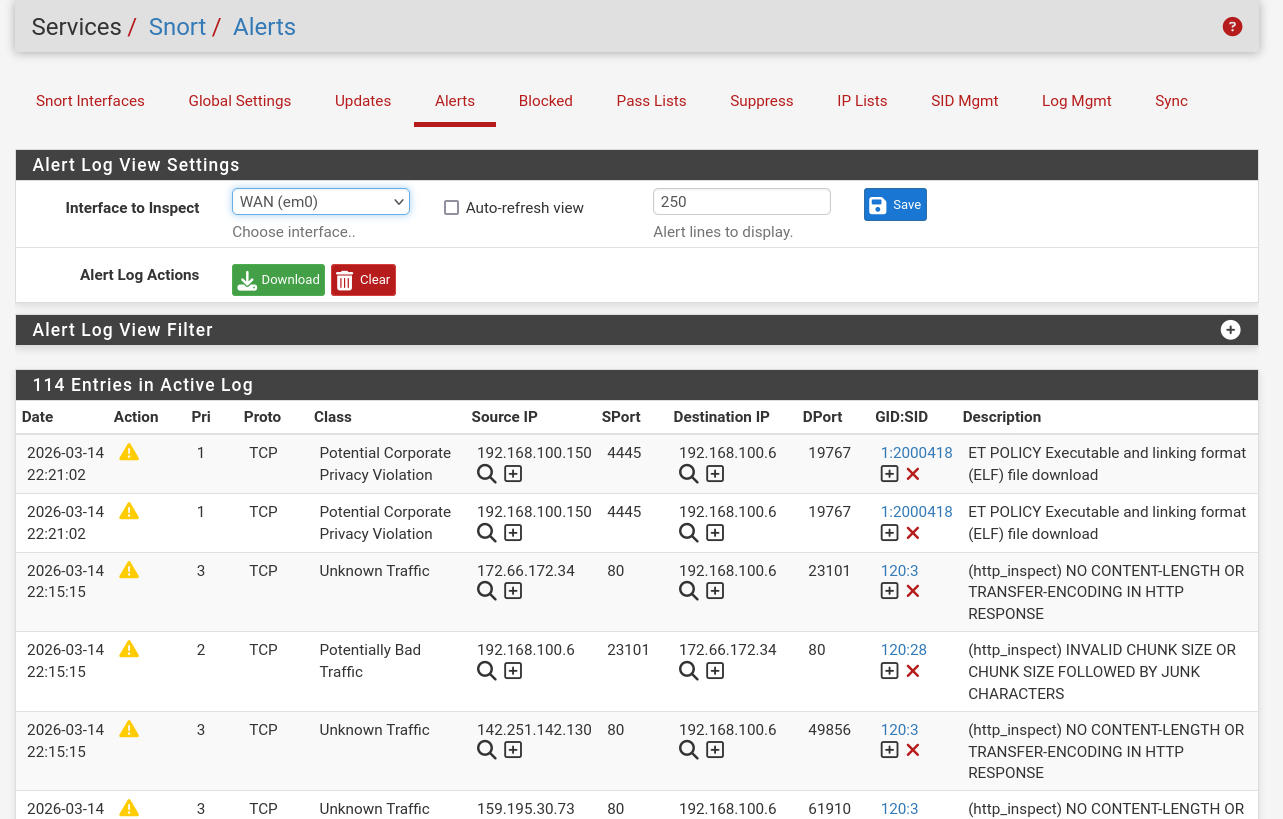
\includegraphics[width=0.98\textwidth]{screenshots/wan-alerts.png}
		\caption{Snort Alerts (WAN) : alertes déclenchées par l'activité depuis 192.168.100.150}
		\label{fig:snort-alerts-wan}
	\end{figure}
	
	\section{Détection sur LAN : mouvement latéral via pivot DMZ}
	
	La figure~\ref{fig:snort-alerts-lan} montre des alertes issues de l'interface \textbf{LAN} (em1). Ce point est critique car il représente ce que les logs du pare-feu ne caractérisent pas nécessairement : une attaque interne issue d'une machine pivot compromise (DMZ).
	
	\subsection{Exemple d'alerte : sonde EternalBlue (MS17-010) détectée}
	
	\begin{lstlisting}[style=logstyle,caption={Extrait d'alerte LAN : détection d'une sonde MS17-010 (EternalBlue) via pivot},label={lst:alert-eternalblue}]
		Date/Time : 2026-03-04 15:28:14
		Interface : LAN (em1)
		Priority  : 1
		Proto     : TCP
		Class     : A Network Trojan was Detected
		Source    : 192.168.10.100:44152
		Dest      : 192.168.20.50:445
		GID:SID   : 1:2025992
		Message   : ET EXPLOIT Possible ETERNALBLUE Probe MS17-010 (Generic Flags)
	\end{lstlisting}
	
	\textbf{Interprétation :}
	\begin{itemize}
		\item La source \textbf{192.168.10.100} correspond au serveur Ubuntu DMZ compromis (pivot).
		\item La destination \textbf{192.168.20.50:445} correspond au poste Windows XP dans le LAN (service SMB).
		\item Snort identifie une signature d'activité typique d'une \textbf{sonde EternalBlue (MS17-010)}.
	\end{itemize}
	
	\textbf{Apport défensif :} cette alerte illustre l'intérêt d'un IDS interne : même si le pare-feu autorise (ou laisse passer via une règle permissive DMZ $\rightarrow$ LAN), Snort fournit un \textbf{contexte d'attaque} et un \textbf{indicateur de compromission} utile aux analystes.
	
	\begin{figure}[H]
		\centering
		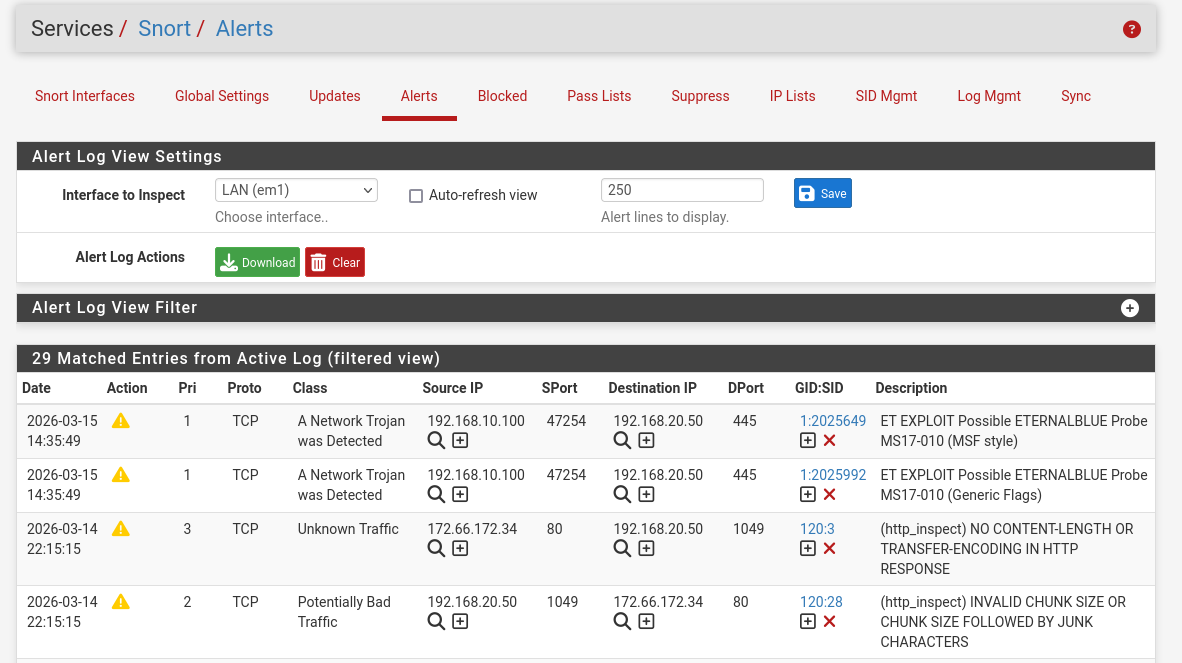
\includegraphics[width=0.98\textwidth]{screenshots/lan-alerts.png}
		\caption{Snort Alerts (LAN) : alertes révélant une activité de mouvement latéral (DMZ $\rightarrow$ LAN)}
		\label{fig:snort-alerts-lan}
	\end{figure}
	
	\section{Discussion : pare-feu vs Snort (visibilité)}
	
	\subsection{Ce que le pare-feu voit}
	Le pare-feu pfSense enregistre qu'un flux a été autorisé entre deux zones selon des règles (IP/ports). Toutefois, un flux autorisé ne signifie pas que son contenu est légitime.
	
	\subsection{Ce que Snort apporte}
	Snort inspecte la charge utile (DPI), compare à des signatures, et produit :
	\begin{itemize}
		\item un horodatage précis,
		\item une classification,
		\item une priorité,
		\item un message décrivant la menace,
		\item un SID permettant l'identification reproductible.
	\end{itemize}
	
	\section{Faux positifs observés et tuning}
	
	Les logs montrent des alertes \texttt{http\_inspect} et des règles de \textit{policy} qui peuvent apparaître en trafic normal, par exemple :
	\begin{itemize}
		\item \texttt{(http\_inspect) NO CONTENT-LENGTH OR TRANSFER-ENCODING IN HTTP RESPONSE}
		\item \texttt{ET POLICY GNU/Linux APT User-Agent Outbound likely related to package management}
	\end{itemize}
	
	\textbf{Approche de tuning recommandée :}
	\begin{enumerate}[leftmargin=*]
		\item Activer uniquement les catégories pertinentes (scan/exploit/samba/web).
		\item Utiliser \textbf{Suppress List} pour des signatures trop bruyantes si elles sont jugées bénignes.
		\item Ajouter des exceptions (\textbf{Pass Lists / IP Lists}) pour des services légitimes.
		\item Envisager l'activation du mode IPS uniquement après stabilisation du tuning.
	\end{enumerate}
	
	% ==============================================================================
	% CHAPITRE 6 : QUESTIONS DE RÉFLEXION
	% ==============================================================================
	\chapter{Questions de Réflexion et Réponses}
	
	\section{Différence fondamentale pare-feu vs IDS/IPS}
	
	\textbf{Réponse :} Un pare-feu filtre principalement sur des métadonnées réseau (IP/ports/protocoles) alors qu'un IDS/IPS analyse le \textbf{contenu} des paquets et la séquence des flux. Un IDS/IPS est plus efficace lorsqu'une attaque transite sur un flux autorisé (ex : SMB autorisé ou mouvement latéral DMZ $\rightarrow$ LAN). Dans notre lab, Snort a détecté une sonde MS17-010 (EternalBlue) alors qu'un pare-feu verrait seulement un flux TCP vers 445.
	
	\section{Comment Snort détecte via signatures (exemple concret)}
	
	\textbf{Réponse :} Snort compare le trafic à des signatures organisées en règles, identifiées par un SID. Une signature décrit un motif d'attaque connu (chaînes, octets, flags, comportements). Exemple observé : \textbf{SID 1:2025992} \textit{ET EXPLOIT Possible ETERNALBLUE Probe MS17-010}. Cette signature a été déclenchée sur un flux \textbf{192.168.10.100} $\rightarrow$ \textbf{192.168.20.50:445}, indiquant une activité SMB suspecte cohérente avec une tentative de détection/exploitation.
	
	\section{Pourquoi la visibilité Snort est cruciale pour le mouvement latéral}
	
	\textbf{Réponse :} Les logs pare-feu montrent des flux autorisés entre zones sans qualifier l'intention. Le mouvement latéral s'effectue souvent à partir d'un pivot interne (DMZ), masquant l'origine externe. Snort sur LAN détecte et alerte sur les motifs d'attaque (ex : sonde EternalBlue) et fournit un contexte (SID, message, priorité), ce que les logs du pare-feu ne donnent pas.
	
	\section{Faux positifs : impacts et gestion}
	
	\textbf{Réponse :} Un faux positif est une alerte déclenchée sur une activité légitime. Trop de faux positifs entraînent une fatigue d'alerte et peuvent masquer les attaques réelles. La gestion repose sur le tuning : désactiver catégories bruyantes, ajuster seuils, utiliser des suppressions ciblées, et n'activer le mode IPS qu'après validation.
	
	% ==============================================================================
	% CHAPITRE 7 : CONCLUSION
	% ==============================================================================
	\chapter{Conclusion et Recommandations}
	
	\section{Bilan}
	
	Ce TP4 a démontré l'apport d'une défense active basée sur IDS :
	\begin{itemize}
		\item Détection sur WAN de comportements et de contenus suspects (ex : transfert de binaire ELF).
		\item Détection sur LAN d'un mouvement latéral depuis la DMZ (ex : sonde MS17-010 / EternalBlue).
		\item Illustration du concept de faux positifs et nécessité du tuning.
	\end{itemize}
	
	\section{Recommandations (production)}
	
	\begin{enumerate}[leftmargin=*]
		\item Passer progressivement vers un mode \textbf{IPS} (blocking) après tuning et validation.
		\item Mettre en place une politique de mise à jour des règles (ET/Snort) et un suivi des alertes prioritaires.
		\item Intégrer les alertes à un SIEM (ELK/Splunk) pour corrélation et réponse à incident.
		\item Restaurer une segmentation stricte : éviter toute règle permissive DMZ $\rightarrow$ LAN en production.
	\end{enumerate}
	
	% ------------------------------------------------------------------------------
	% ANNEXES (optionnel)
	% ------------------------------------------------------------------------------
	\appendix
	\chapter{Annexes : Captures et Preuves}
	
	\begin{tcolorbox}[colback=primary!5!white, colframe=primary, title=\textbf{Fichiers requis dans le dossier du projet LaTeX}]
		Pour compiler sans erreur, placer les images suivantes dans le même dossier que ce fichier :
		\begin{itemize}
			\item \texttt{snort-interfaces.png} (capture Snort Interfaces : WAN/DMZ/LAN running)
			\item \texttt{snort-global-settings.png} (capture Global Settings : GPLv2 + ET Open)
						\item \texttt{wan-alerts.png} (capture Alerts filtrée WAN)
			\item \texttt{lan-alerts.png} (capture Alerts filtrée LAN)
			\end{itemize}
		\end{tcolorbox}
	
\section{Index des preuves (références rapides)}

\begin{table}[H]
\centering
\renewcommand{\arraystretch}{1.4}
\setlength{\arrayrulewidth}{0.5pt}
\begin{tabular}{p{3.2cm} p{5.2cm} p{6.2cm}}
\arrayrulecolor{tableborder}
\hline
\tableheadcolor
\textcolor{tableheadfg}{\textbf{Élément}} &
\textcolor{tableheadfg}{\textbf{Preuve}} &
\textcolor{tableheadfg}{\textbf{Localisation dans le rapport}} \\
\hline
\rowcolor{tablerowalt}
Interfaces Snort & \texttt{snort-interfaces.png} & Fig.~\ref{fig:snort-interfaces} \\
Sources de règles & \texttt{snort-global-settings.png} & Fig.~\ref{fig:snort-global-settings} \\
\rowcolor{tablerowalt}
Alertes WAN & \texttt{wan-alerts.png} & Fig.~\ref{fig:snort-alerts-wan} + List.~\ref{lst:alert-elf} \\
Alertes LAN & \texttt{lan-alerts.png} & Fig.~\ref{fig:snort-alerts-lan} + List.~\ref{lst:alert-eternalblue} \\
\hline
\end{tabular}
\caption{Index des preuves et ancrages dans le rapport}
\label{tab:evidence-index}
\end{table}

\section{Commentaires sur la reproductibilité}

\subsection{Paramètres critiques}

Pour reproduire ce TP dans un environnement identique, les paramètres suivants doivent être strictement respectés :
\begin{itemize}
\item \textbf{Segmentation réseau} : trois sous-réseaux distincts (WAN/DMZ/LAN).
\item \textbf{Plan d'adressage} : cohérent avec la Table~\ref{tab:ip-plan-tp4}.
\item \textbf{Règles pfSense} : présence des redirections NAT (WAN $\rightarrow$ DMZ) et, pour la partie pédagogique \textit{pivoting}, existence d'une règle permissive (DMZ $\rightarrow$ LAN) \textbf{uniquement en laboratoire}.
\item \textbf{Règles Snort} : activation de \textbf{Snort GPLv2} et \textbf{ET Open}, et sélection de catégories pertinentes (scan / exploit / netbios-smb / web).
\end{itemize}

\subsection{Limites connues}

\begin{itemize}
\item \textbf{Trafic chiffré (HTTPS)} : Snort ne peut pas inspecter le contenu applicatif sans mécanisme de déchiffrement (non mis en place dans ce TP).
\item \textbf{Signatures} : détection très efficace sur menaces connues, mais limitée face aux attaques zero-day.
\item \textbf{Faux positifs} : présence d'alertes \textit{policy} et \textit{http\_inspect} démontrant la nécessité d'un tuning pour exploitation en production.
\end{itemize}

\section{Annexe A : Résumé des alertes exploitées (extraits)}

\begin{longtable}{p{2.8cm} p{1.2cm} p{2.3cm} p{4.1cm} p{4.1cm}}
\arrayrulecolor{tableborder}
\hline
\tableheadcolor
\textcolor{tableheadfg}{\textbf{Horodatage}} &
\textcolor{tableheadfg}{\textbf{Pri}} &
\textcolor{tableheadfg}{\textbf{SID}} &
\textcolor{tableheadfg}{\textbf{Flux (SRC $\rightarrow$ DST)}} &
\textcolor{tableheadfg}{\textbf{Message}} \\
\hline
\endfirsthead

\hline
\tableheadcolor
\textcolor{tableheadfg}{\textbf{Horodatage}} &
\textcolor{tableheadfg}{\textbf{Pri}} &
\textcolor{tableheadfg}{\textbf{SID}} &
\textcolor{tableheadfg}{\textbf{Flux (SRC $\rightarrow$ DST)}} &
\textcolor{tableheadfg}{\textbf{Message}} \\
\hline
\endhead

\hline
\multicolumn{5}{r}{\small\textcolor{footergray}{Suite à la page suivante}}\\
\endfoot

\hline
\endlastfoot

\rowcolor{tablerowalt}
2026-03-14 22:21:02 & 1 & 1:2000418 &
192.168.100.150:4445 $\rightarrow$ 192.168.100.6:19767 &
ET POLICY Executable and linking format (ELF) file download \\

2026-03-04 15:28:14 & 1 & 1:2025992 &
192.168.10.100:44152 $\rightarrow$ 192.168.20.50:445 &
ET EXPLOIT Possible ETERNALBLUE Probe MS17-010 (Generic Flags) \\
\end{longtable}

\begin{tcolorbox}[colback=secondary!5!white, colframe=secondary, title=\textbf{Note méthodologique}]
Les deux alertes ci-dessus ont été retenues car elles couvrent les deux dimensions attendues du TP4 :
\begin{itemize}
\item \textbf{WAN (périmètre)} : visibilité sur une action offensive depuis l'attaquant (payload ELF).
\item \textbf{LAN (interne)} : visibilité sur une tentative de mouvement latéral depuis le pivot DMZ vers Windows XP (SMB/445).
\end{itemize}
\end{tcolorbox}

% ------------------------------------------------------------------------------
% FIN DU DOCUMENT
% ------------------------------------------------------------------------------
\end{document}
